\documentclass[conference]{IEEEtran}
\usepackage{cite}
\usepackage{amsmath,amssymb,amsfonts}
\usepackage{algorithmic}
\usepackage{graphicx}
\usepackage{textcomp}
\usepackage{xcolor}
\usepackage{pgfplots}
\pgfplotsset{compat=1.18}

\usepackage{tikz}
\usetikzlibrary{arrows.meta, positioning, shapes.geometric}

\begin{document}

\title{The Calçotada Protocol: \ Equity Peg Tokens for Decentralized Venture Capital}

\author{\IEEEauthorblockN{Author Name}
\IEEEauthorblockA{\textit{Organization} \\
City, Country \\
email@example.com}}

\maketitle

\begin{abstract}
This paper presents the Calçotada Protocol, a blockchain-based framework for democratizing early-stage venture capital through tokenized convertible notes designed to track startup valuations. The protocol implements a dual-token architecture combining ERC721 NFTs for governance participation with ERC20 RMSC tokens for economic exposure. Built on Polygon with Chainlink oracle integration, the system features sophisticated bonding curve pricing, automated treasury management, and transparent on-chain fundraising mechanics. While the current implementation provides core token infrastructure, future development will add on-chain accountancy, automated buyback mechanisms, and full DAO governance to create a complete decentralized venture capital platform accessible to retail investors.
\end{abstract}

\begin{IEEEkeywords}
Blockchain, Venture Capital, Decentralized Finance, Tokenization, Equity Peg Token, DAO
\end{IEEEkeywords}

\section{Introduction: Unlocking Foundational Capital for Everyone}

Venture capital (VC) acts simultaneously as the engine and gatekeeper of innovation, deciding which startups receive funding and consequently determining who shapes the products and services of tomorrow. This concentration of influence leads to what Acemoglu and Johnson describe as a "tunnel vision" in their seminal work \textit{Power and Progress} (2023), wherein the future is shaped not by societal necessities or disruptive innovations, but by trends favored by large capital holders. This cycle perpetuates itself: venture capital firms backed by substantial resources dictate innovation agendas, consolidating wealth and reinforcing their dominance over technological and economic progress.

This entrenched model of early-stage investing not only restricts innovation to predefined agendas but exacerbates inequality by excluding smaller investors from the highest-return investment opportunities—namely, seed-stage equity rounds. Consequently, retail investors resort to speculative assets such as memecoins, seeking the kinds of outsized returns historically realized in early-stage VC funding, but without genuine exposure to underlying innovation or governance rights.

Blockchain technology offers a foundational shift in this dynamic by enabling decentralized autonomous organizations (DAOs) and token-based governance models to democratize access to venture-stage capital and decision-making processes.

The Calçotada Protocol is our practical response to this systemic imbalance. It presents a vision for structured, transparent on-chain mechanisms that will link token ownership to startup valuations and governance rights. Through tokenized convertible notes, the protocol aims to allow individual investors—not just large institutions—to meaningfully participate in both the financial and governance aspects of promising startups at their earliest stages.

This whitepaper presents both the current Minimum Viable Product (MVP) implementation and the complete protocol vision. The MVP, consisting of 333 Genesis NFTs and foundational smart contracts, serves as a proof of concept and market validation tool. With a modest target of €30,000, this initial phase focuses on validating interest, building a core team, and establishing fundamental protocol standards before expanding to the full implementation.

The protocol was specifically developed to meet the funding requirements of The Calçotada Company, a food-tech startup with a disruptive and validated business model. This measured approach—starting with an MVP and growing based on community feedback—ensures that the protocol development remains aligned with real market needs while building the foundation for Decentralized Autonomous Venture Capital (DAVC).

\section{Prior Art and Related Work}

Blockchain technology has significantly altered the landscape of startup financing, leading to an emergence of novel funding mechanisms primarily through Initial Coin Offerings (ICOs) and token sales. Guangye Cao (2023), in his seminal paper \textit{``Startup Financing: Token vs Equity"}, highlights that blockchain-based startups commonly prefer token issuance over traditional equity due to enhanced liquidity and lower return expectations from investors, driven by early liquidity rather than intrinsic valuation \cite{cao2023token}. However, this financing model predominantly targets crypto-native startups building decentralized applications (dApps) or blockchain protocols. Thus, these tokens typically derive value from speculative market dynamics rather than a measurable relationship to company success or valuation milestones \cite{howell2020initial, catalini2019some}.

Several foundational studies underline these market dynamics. Howell et al. (2020) find that token success in ICOs correlates closely with disclosure practices and speculative expectations rather than fundamental valuation metrics tied explicitly to a startup’s success \cite{howell2020initial}. Similarly, Chod and Lyandres (2021) point out that token financing frequently introduces agency problems, as entrepreneurs are incentivized to underproduce since their revenues are not strictly pegged to token values or vice versa \cite{chod2021theory}. Cong et al. (2021) also note the prevalence of speculative pricing, driven largely by investor expectations about future platform popularity rather than underlying business fundamentals \cite{cong2021tokenomics}.

The literature further emphasizes a structural shortcoming in current token funding models, specifically their inherent inability to effectively bridge token valuation to real-world company performance and equity milestones. For example, the widely-used Simple Agreement for Future Tokens (SAFT), while attempting to integrate traditional funding elements, still ultimately relies on future speculative market conditions rather than measurable startup outcomes \cite{mendelson2019saft}. Meanwhile, token-warrant structures and automated convertible notes introduced by ConsenSys and others attempt to blend equity and token economics but do not provide explicit pegging mechanisms between token value and company valuation, leaving substantial room for market speculation and volatility \cite{lw2019token}.

In this context, token financing as historically implemented has primarily appealed to blockchain-focused ventures, offering limited utility to traditional non-crypto enterprises seeking structured and valuation-based early-stage financing mechanisms. Despite clear liquidity advantages outlined by Cao (2023) and others, the absence of a stable and measurable peg to equity valuation remains a critical gap in current blockchain funding structures.

Addressing precisely this gap, the Calçotada Protocol proposes an innovative framework: a \textit{Tokenized Convertible Note (TCN)} explicitly pegged to company valuation. By bridging traditional valuation-linked financial instruments with blockchain-enabled liquidity, the protocol uniquely positions itself as a solution capable of transcending speculative market dynamics and offering structured equity participation and governance rights to retail investors.

\section{Extended Analysis of Dual-Token Models}

\subsection{Dual-Asset Token Models}

A growing class of decentralized finance and DAO systems use a dual-token model, combining:

\begin{itemize}
    \item A non-fungible or governance token for voting/access
    \item A fungible token for utility or financial participation
\end{itemize}

Examples include:

\textbf{Charged Particles} offers a framework allowing NFTs to hold fungible tokens—creating hybrid assets, but not necessarily valuation‑pegged economic instruments~\cite{chargedparticles2022}.

\textbf{Tensor DAO} issues a governance token (TNSR) alongside protocol usage tokens—holders vote and receive revenue-share—but tokens are not directly pegged to outside company valuations~\cite{tensor2025}.

\textbf{Origyn Protocol} uses OGY as a fungible utility/governance token alongside provenance NFTs—though again, without a peg to company performance~\cite{origyn2022}.

Academic work on NFT authentication and hybrid structures exists (e.g. Talgar \& Banach~\cite{talgar2024dao}, Avrilionis \& Hardjono~\cite{avrilionis2022assetproxy}), but these focus on access control or metadata consistency—not on funding mechanics or value-redemption.

\subsection{Research Gap}

While dual-token models are gaining traction in DeFi and NFT ecosystems, none explicitly link the fungible token’s value to company performance or guarantee redemption pegged to valuation. Existing models focus on speculative pricing, membership perks, or governance, not on treating tokens as digital equity with built-in mechanisms to ensure economic alignment.

\subsection{Contribution of the Calçotada Protocol}

The Calçotada Protocol bridges these gaps by:

\begin{itemize}
    \item Issuing \textbf{Founder NFTs} for governance and access;
    \item Issuing \textbf{RMSC fungible tokens} with a strict, externally validated PEG to company valuation;
    \item Enforcing buyback commitments on-chain via transparent smart contracts and external oracles;
    \item Combining liquidity, governance, and valuation parity in a single dual-token financial architecture.
\end{itemize}



\section{Fundamental Key Assets and On-Chain Accountancy}
A primary innovation of the Calçotada Protocol is the incorporation of on-chain accountancy as a transparent foundation for venture valuations, investor returns, and protocol trust. This section reviews the strategic assets necessary for protocol integrity and public confidence, highlighting how on-chain financial tracking directly informs estimated valuations and buyback commitments.

\subsection{On-Chain Accountancy}
Unlike traditional venture frameworks—where assessment of company value and investor ROI rely on opaque, often delayed financial reporting—the Calçotada Protocol mandates continuous, verifiable financial accounting on-chain. All critical financial flows (revenue, costs, operational reserves, distributions) are recorded in transparent smart contracts.

This enables:
\begin{itemize}
    \item \textbf{Real-time, tamper-proof valuation:} Investors and protocol governors can view up-to-date figures at any point, reducing ambiguity or information asymmetry.
    \item \textbf{Reliable ROI estimates:} Using industry-standard financial metrics (see next subsection), the protocol can project and periodically update company valuations and potential ROI for token holders.
    \item \textbf{Algorithmic buyback triggers:} Token buyback amounts and conditions are derived from on-chain accounting data, automating investor returns and aligning incentives.
\end{itemize}

\subsection{Valuation Methodology and Financial Modeling}
To ensure that buybacks reflect fundamentally justified valuations, the protocol leverages conventional startup valuation techniques. The accompanying \texttt{Tokenomics RMSC.ods} model calculates buyback scenarios and expected valuations based on revenue multiples, discounted cash flows, or other startup-typical factors. These methods are encoded in oracles or contract formulas, supporting automated, auditable financial flows without need for off-chain negotiations.

This structure allows retail and institutional investors to benefit from return estimates and exit strategies anchored in both blockchain transparency and accepted financial practice—even before actual company liquidity events.

\subsection{Additional Key Assets}
\begin{itemize}
    \item \textbf{Smart Contracts:} All protocol commitments (NFTs, RMSC tokenomics, buybacks, treasury reserve) are transparently on-chain.
    \item \textbf{External Oracles:} For validation of off-chain revenue or event triggers as needed.
    \item \textbf{Decentralized Governance:} Founder NFTs enable participatory protocol upgrades and control structures.
\end{itemize}

\section{Protocol Architecture}

\usetikzlibrary{arrows.meta, positioning, shapes.geometric}

\begin{figure}[ht]
\centering
\scalebox{0.5}{%
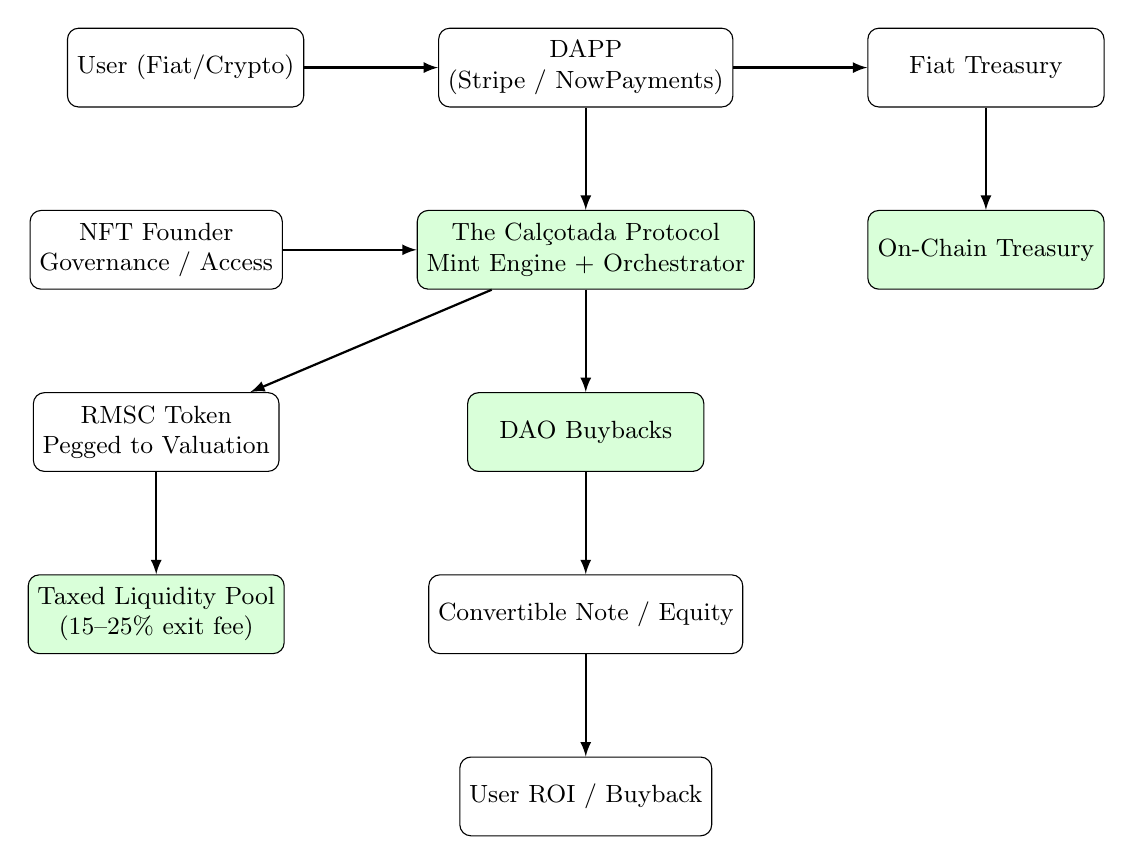
\begin{tikzpicture}[node distance=1.3cm and 1.7cm, every node/.style={font=\small}]

% Styles
\tikzstyle{box} = [draw, rounded corners, align=center, minimum width=3cm, minimum height=1cm, fill=white]
\tikzstyle{greenbox} = [box, fill=green!15]
\tikzstyle{arrow} = [->, thick, >=latex]

% Nodes
\node[box] (user) {User (Fiat/Crypto)};
\node[box, right=of user] (dapp) {DAPP\\(Stripe / NowPayments)};
\node[box, right=of dapp] (fiat) {Fiat Treasury};
\node[greenbox, below=of fiat] (onchain) {On-Chain Treasury};

\node[greenbox, below=of dapp] (protocol) {The Calçotada Protocol\\Mint Engine + Orchestrator};

\node[box, left=of protocol] (nft) {NFT Founder\\Governance / Access};
\node[box, below=of nft] (rmsc) {RMSC Token\\Pegged to Valuation};

\node[greenbox, below=of protocol] (dao) {DAO Buybacks};
\node[box, below=of dao] (equity) {Convertible Note / Equity};
\node[box, below=of equity] (payback) {User ROI / Buyback};

\node[greenbox, below=of rmsc] (tlp) {Taxed Liquidity Pool\\(15–25\% exit fee)};

% Arrows
\draw[arrow] (user) -- (dapp);
\draw[arrow] (dapp) -- (fiat);
\draw[arrow] (fiat) -- (onchain);
\draw[arrow] (dapp) -- (protocol);

\draw[arrow] (nft) -- (protocol);
\draw[arrow] (protocol) -- (rmsc);
\draw[arrow] (protocol) -- (dao);
\draw[arrow] (dao) -- (equity);
\draw[arrow] (equity) -- (payback);
\draw[arrow] (rmsc) -- (tlp);

\end{tikzpicture}%
}%
\caption{Simplified architecture of the Calçotada Protocol: dual-token issuance and treasury-integrated valuation peg.}
\end{figure}

% 
\usepackage{tikz-uml}

\begin{figure}[ht]
\centering
\scalebox{0.5}{%
\begin{tikzpicture}[node distance=1.6cm and 1.8cm]

% LEFT COLUMN
\node (rmsc) [tokencontract] {RMSCToken \nodepart{second} ERC20 \\ Peg Mechanism \nodepart{third} mint() \\ burn() \\ buyback()};
\node (nft) [tokencontract, below=of rmsc] {FounderNFT \nodepart{second} ERC721 \\ Governance \nodepart{third} vote() \\ access()};

% CENTER
\node (protocol) [orchestrator, right=of rmsc, yshift=-1cm] {THE CALÇOTADA \nodepart{second} Orchestrator \\ Mint Engine \nodepart{third} Controller Functions};

% RIGHT
\node (fiatinput) [treasurycontract, above=of protocol] {FiatInputContract \nodepart{second} Deposit \nodepart{third} Withdraw};
\node (onchain) [treasurycontract, below=0.8cm of fiatinput] {OnChainTreasury \nodepart{second} Store \nodepart{third} Audit};
\node (paytreasury) [treasurycontract, right=of fiatinput] {PaydayTreasury \nodepart{second} Pay \nodepart{third} Distribute};

\node (daobuybacks) [contract, right=of protocol, yshift=-1cm] {DAOBuybacks \nodepart{second} Convertible Note \\ SAFE + Equity \nodepart{third} execute() \\ validate()};
\node (daotube) [contract, right=of daobuybacks] {DAOTube \nodepart{second} Buyback Handler \nodepart{third} process() \\ distribute()};
\node (instruments) [contract, below=of daotube] {Instruments \nodepart{second} Financial Tools \nodepart{third} convert() \\ redeem()};
\node (userwallet) [contract, below=of instruments] {UserWallet \nodepart{second} Balance Manager \nodepart{third} deposit() \\ withdraw()};

% BOTTOM
\node (taxpool1) [treasurycontract, below=of nft, xshift=3cm] {TaxedLiquidityPool \nodepart{second} Exit Tax Handler \nodepart{third} collect() \\ redistribute()};
\node (taxpool2) [treasurycontract, below=of daobuybacks] {TaxedLiquidityPool \nodepart{second} Exit Tax Handler \nodepart{third} collect() \\ redistribute()};

% ARROWS
\draw [arrow] (fiatinput) -- (onchain);
\draw [arrow] (fiatinput) -- (paytreasury);
\draw [arrow] (paytreasury) |- (daotube);
\draw [arrow] (onchain) -- (protocol);

\draw [arrow] (rmsc) -- (protocol);
\draw [arrow] (nft) -- (protocol);

\draw [arrow] (protocol) -- (daobuybacks);
\draw [arrow] (daobuybacks) -- (daotube);
\draw [arrow] (daotube) -- (instruments);
\draw [arrow] (instruments) -- (userwallet);

\draw [arrow] (protocol) -- (taxpool1);
\draw [arrow] (daobuybacks) -- (taxpool2);

\end{tikzpicture}%
}%
\caption{Calçotada Protocol smart contract architecture: UML-style representation showing contract classes, interfaces, and function signatures for the dual-token system.}
\end{figure}


The Calçotada Protocol implements a sophisticated two-asset system deployed on the Polygon blockchain to facilitate decentralized venture funding. The architecture consists of four core smart contracts that work in concert: CalcotCoin (NFT), Romesco (RMSC token), Calçotada (orchestrator), and NormalizeToEuro (oracle integration). This system combines governance through non-fungible tokens (NFTs) with economic participation via fungible tokens (RMSC) that are designed to track company valuation.

\subsection{CalcotCoin NFT: Governance and Foundational Access}

The \textit{CalcotCoin} (CEBA) contract implements an ERC721 NFT system designed to recognize early supporters and provide governance rights. The current implementation features:

\textbf{Technical Specifications:}
\begin{itemize}
    \item Fixed supply of 333 NFTs (CEBA Genesis edition)
    \item 33 tokens reserved for treasury (10\% allocation)
    \item Linear pricing mechanism from 222.22 to 200 RMSC per NFT
    \item Base price of 100 EUR per NFT with dynamic RMSC conversion
\end{itemize}

\textbf{Minting Mechanism:}
The CalcotCoin contract implements a sophisticated dual-minting system where NFT purchases trigger a 2x RMSC mint. When purchasing an NFT:
\begin{enumerate}
    \item The buyer receives 2x the NFT price in newly minted RMSC
    \item Half of the RMSC is automatically transferred to the treasury as payment
    \item The buyer retains the other half as a bonus incentive
    \item The NFT is minted to the buyer's address
\end{enumerate}

\textbf{Planned Governance Features:}
\begin{itemize}
    \item One vote per wallet (implementation pending)
    \item Participation in valuation recognition and capital allocation decisions
    \item Access to exclusive founder communications
\end{itemize}

Note: The whitepaper originally specified 6 batches totaling 5,888 NFTs. The current implementation focuses on the initial 333-unit genesis collection, with future batches to be deployed based on protocol evolution and community feedback.

\subsection{RMSC Token: Equity-Pegged Financial Instrument}

The \textit{Romesco Token (RMSC)} is the core financial instrument of the protocol, implemented as an ERC20 token with ERC1363 and ERC20Permit extensions for enhanced functionality.

\textbf{Technical Implementation:}
\begin{itemize}
    \item Fixed maximum supply of 5,000,000 RMSC (hard cap enforced in contract)
    \item Initial pre-mint of 200,000 RMSC for liquidity and operational needs
    \item Pausable functionality for emergency situations
    \item Permit functionality for gasless approvals
    \item ERC1363 support for single-transaction transfers and callbacks
\end{itemize}

\textbf{Economic Design:}
\begin{itemize}
    \item Minting controlled by the orchestrator contract only
    \item No burn functionality for regular users (maintains supply integrity)
    \item Designed for future buyback mechanism at €1.5–€3.0 per RMSC
    \item Starting valuation implies approximately €0.40–€0.60 per RMSC
\end{itemize}

\textbf{Integration Features:}
The RMSC token is designed for composability with DeFi protocols:
\begin{itemize}
    \item ERC20Permit enables gasless transactions and meta-transactions
    \item ERC1363 allows for advanced payment flows and automated callbacks
    \item Standard ERC20 interface ensures compatibility with all major DEXs and lending protocols
\end{itemize}

Note: The buyback mechanism mentioned in the economic design is planned for future implementation through a separate contract that will interact with the on-chain accountancy system.

\subsection{Calçotada Orchestrator: Protocol Coordination}

The \textit{Calçotada} contract serves as the central orchestrator, coordinating interactions between all protocol components:

\textbf{Core Functions:}
\begin{itemize}
    \item Manages the dual-minting mechanism for NFT purchases
    \item Controls RMSC minting according to bonding curve pricing
    \item Handles both public and private sale mechanisms
    \item Integrates with NormalizeToEuro for multi-currency support
\end{itemize}

\textbf{Bonding Curve Implementation:}
The orchestrator implements a sophisticated normalized bonding curve using:
\begin{itemize}
    \item Q16.16 fixed-point arithmetic for precision
    \item Configurable sigmoid curve shape for optimal price discovery
    \item Integration with trapezoidal rule for accurate pricing
    \item Starting price: €0.40 per RMSC, ending price: €0.60 per RMSC
\end{itemize}

\textbf{Transaction Fee Structure:}
\begin{itemize}
    \item NFT purchases: €4.50 transaction fee
    \item RMSC purchases: €2.50 transaction fee
    \item Fees collected in POL and forwarded to treasury
\end{itemize}

\subsection{Price Oracle Integration}

The \textit{NormalizeToEuro} contract provides real-time price conversion using Chainlink oracles:

\textbf{Oracle Feeds:}
\begin{itemize}
    \item ETH/USD, EUR/USD, and POL/USD price feeds
    \item Automatic conversion between EUR pricing and POL payments
    \item 18-decimal precision for all calculations
\end{itemize}

\subsection{PEG Enforcement and Future Development}

While the current implementation provides the foundation for equity-pegged tokens, the full PEG mechanism awaits implementation:

\textbf{Current State:}
\begin{itemize}
    \item Token supply and pricing mechanisms are fully implemented
    \item Oracle integration provides real-time price conversion
    \item Treasury accumulation occurs automatically
\end{itemize}

\textbf{Planned Enhancements:}
\begin{itemize}
    \item On-chain accountancy module for transparent financial tracking
    \item Automated buyback contracts triggered by valuation milestones
    \item Governance voting mechanisms for NFT holders
    \item Integration with external valuation attestation services
\end{itemize}

\subsection{Initial Supply and Distribution}

The initial supply of RMSC tokens is allocated in a controlled and transparent manner to recognize pre-protocol contributions and prepare for public issuance. No tokens are minted speculatively or granted without capital justification.

\subsubsection{Angel Investor Allocation}

Prior to the protocol's launch, a group of early angel investors provided capital to The Calçotada Company under a convertible loan agreement. These early backers are entitled to receive RMSC tokens at the protocol’s base issuance price, plus an interest premium to account for the time value of their risk.

\begin{itemize}
    \item \textbf{Base Price Conversion:} Angel investments are converted into RMSC at the same base price offered during the initial public issuance phase.
    \item \textbf{Interest Adjustment:} A fixed 7\% interest rate is applied to the original invested amount, and this adjusted total determines the corresponding RMSC allocation.
    \item \textbf{Non-inflationary Grant:} These tokens are accounted for as part of the protocol's total capped supply and are not created in excess of the 5 million RMSC ceiling.
\end{itemize}

\subsubsection{Pre-Mint Reserve}

In addition to angel investor conversion, a total of 200,000 RMSC tokens are pre-minted and held in the protocol treasury for operational, liquidity, and market stabilization purposes. This reserve will be used judiciously to support exchange listings, liquidity pool seeding, and strategic partnerships.

\subsubsection{Public Issuance}

All remaining RMSC tokens are made available through direct, capital-backed purchase via the protocol interface. Tokens are minted on-demand as described in the Minting Scheme, with no pre-sale, airdrop, or speculative allocation.

This initial supply model ensures that token distribution is fully aligned with the company’s real financial history and avoids the common pitfalls of over-allocation, unbacked inflation, or opaque private rounds.

\subsection{Initial Distribution and Structured Pricing}

The protocol implements a sophisticated pricing mechanism that balances early adopter incentives with sustainable fundraising:

\subsubsection{Current Implementation: Genesis Collection}

The deployed contracts focus on the initial CalcotCoin Genesis collection:
\begin{itemize}
    \item 333 total NFTs with 33 reserved for treasury
    \item Linear RMSC pricing from 222.22 to 200 RMSC per NFT
    \item Fixed EUR price of €100 per NFT
    \item Dual-minting mechanism providing 2x RMSC to NFT buyers
\end{itemize}

\subsubsection{Future Batch Structure}

The protocol design accommodates future expansion through additional NFT collections:

\begin{table}[ht]
\caption{NFT Batches and Associated RMSC Minting}
\centering
\scriptsize
\begin{tabular}{|p{1.5cm}|p{0.6cm}|p{0.7cm}|p{0.7cm}|p{0.7cm}|}
\hline
\textbf{Batch} & \textbf{NFTs} & \textbf{NFT €} & \textbf{RMSC €} & \textbf{MINT kRMSC} \\
\hline
Calçot Coins     & 333  & 100  & 0.40  & 66  \\
FounderPass 1    & 555  & 125  & 0.50  & 139  \\
FounderPass 2    & 1111 & 250  & 0.525 & 529  \\
FounderPass 3    & 1111 & 375  & 0.55  & 757  \\
FounderPass 4    & 1111 & 500  & 0.575 & 966  \\
FounderPass 5    & 1111 & 625  & 0.60  & 1,157  \\
\hline
\multicolumn{5}{|c|}{\textbf{Total: 5,332 NFTs}} \\
\multicolumn{5}{|c|}{\textbf{2,047,025 € raised, 1,807,796 RMSC minted}} \\
\hline
\end{tabular}
\end{table}






Half of the RMSC minted for each NFT is transferred to the protocol treasury, while the remaining half is consumed by the NFT minting contract. This ensures that treasury-backed liquidity grows proportionally with capital raised.

\subsubsection{Public RMSC Issuance via Bonding Curve}

The Calçotada orchestrator implements a sophisticated bonding curve mechanism for public RMSC sales:

\textbf{Technical Implementation:}
\begin{itemize}
    \item Normalized sigmoid curve stored as Q16.16 fixed-point values
    \item Configurable curve shape via uploadable parameters
    \item 16-step trapezoidal integration for accurate pricing
    \item Real-time POL/EUR conversion via Chainlink oracles
\end{itemize}

\textbf{Pricing Parameters:}
\begin{itemize}
    \item Starting price: €0.40 per RMSC
    \item Ending price: €0.60 per RMSC  
    \item Available supply: Up to 4.6M RMSC (after pre-mint and NFT allocations)
    \item Transaction fee: €2.50 per purchase
\end{itemize}
\begin{figure}[ht]
\centering
\begin{tikzpicture}
\begin{axis}[
    width=\linewidth,
    height=6cm,
    grid=both,
    xlabel={\textbf{Fraction of Supply Minted}},
    ylabel={\textbf{RMSC Price (€)}},
    title={Sigmoid Bonding Curve for Public RMSC Issuance},
    ymin=39, ymax=61,
    xmin=0, xmax=1,
    thick
]
\addplot[
    color=blue,
    mark=none
]
table[
    col sep=comma,
    x=fraction_minted,
    y=rmsc_price_eur
] {rmsc_sigmoid_curve.csv};
\end{axis}
\end{tikzpicture}
\caption{Sigmoid bonding curve used for public RMSC issuance pricing.}
\label{fig:sigmoidcurve}
\end{figure}



This curve allows the protocol to capture higher marginal funding value while maintaining a predictable and fair pricing structure. Early public buyers enjoy lower prices, and late-stage buyers pay a premium as the available supply nears exhaustion.

\subsubsection{Liquidity and Secondary Market Strategy}

The protocol's liquidity strategy leverages standard DeFi infrastructure:

\textbf{Current Implementation:}
\begin{itemize}
    \item RMSC is a standard ERC20 token, compatible with all major DEXs
    \item Treasury accumulates POL and RMSC for future liquidity provision
    \item No transfer restrictions or vesting schedules
\end{itemize}

\textbf{Planned Liquidity Features:}
\begin{itemize}
    \item DEX liquidity pools on QuickSwap or Uniswap V3
    \item Treasury-funded initial liquidity provision
    \item Potential liquidity mining incentives for early providers
    \item Integration with lending protocols for RMSC collateralization
\end{itemize}

Note: The Taxed Liquidity Pool (TLP) mentioned in the original design is deferred to future protocol upgrades, allowing for simpler initial deployment and community-driven liquidity solutions.


\subsection{Network Deployment}

Polygon is selected as the base network for its:
\begin{itemize}
    \item Low transaction fees and fast confirmation times,
    \item Proven security track record via Ethereum finality,
    \item Established ecosystem of NFT and DeFi projects.
\end{itemize}

Deploying on Polygon enables frictionless user participation while ensuring composability with future liquidity protocols and DAO tools.



\section{Technical Implementation}

\subsection{Smart Contract Architecture}

The Calçotada Protocol consists of four core smart contracts deployed on Polygon:

\textbf{1. CalcotCoin.sol (ERC721):}
\begin{itemize}
    \item Manages NFT issuance and ownership
    \item Implements linear pricing mechanism
    \item Handles treasury pre-allocation
    \item Integrates with orchestrator for minting
\end{itemize}

\textbf{2. Romesco.sol (ERC20):}
\begin{itemize}
    \item Implements capped token supply (5M RMSC)
    \item Provides ERC1363 and Permit extensions
    \item Controlled minting via orchestrator only
    \item Pausable for emergency situations
\end{itemize}

\textbf{3. Calcotada.sol (Orchestrator):}
\begin{itemize}
    \item Coordinates all protocol interactions
    \item Implements bonding curve pricing
    \item Manages dual-minting mechanism
    \item Handles fee collection and treasury forwarding
\end{itemize}

\textbf{4. NormalizeToEuro.sol (Oracle):}
\begin{itemize}
    \item Integrates Chainlink price feeds
    \item Provides EUR/POL/ETH conversions
    \item Ensures accurate multi-currency pricing
\end{itemize}

\subsection{Security Considerations}

\textbf{Access Control:}
\begin{itemize}
    \item Owner-controlled administrative functions
    \item Orchestrator pattern for inter-contract calls
    \item No external minting access on token contracts
\end{itemize}

\textbf{Safety Features:}
\begin{itemize}
    \item ReentrancyGuard on all payment functions
    \item Pausable functionality for emergency response
    \item Overflow protection via Solidity 0.8.28
    \item Battle-tested OpenZeppelin libraries
\end{itemize}

\subsection{Gas Optimization}

\begin{itemize}
    \item Batch minting reduces per-NFT gas costs
    \item Q16.16 arithmetic minimizes computational overhead
    \item Efficient storage patterns in bonding curve
    \item Optimized loops with unchecked arithmetic where safe
\end{itemize}

\section{Conclusion and Future Work}

The Calçotada Protocol represents a significant step toward democratizing venture capital through blockchain technology. By implementing tokenized convertible notes with clear valuation pegs, the protocol creates a bridge between traditional startup funding and decentralized finance.

\subsection{Current MVP Implementation}

The deployed Minimum Viable Product serves as a proof of concept and market validation tool:

\textbf{Implemented Features:}
\begin{itemize}
    \item Genesis collection of 333 CalçotCoin NFTs at €100 each
    \item RMSC token with 5M supply cap and bonding curve mechanics
    \item Dual-minting system rewarding early supporters
    \item Oracle integration for EUR/POL price conversion
    \item Basic treasury accumulation mechanism
\end{itemize}

\textbf{MVP Objectives:}
\begin{itemize}
    \item Demonstrate technical feasibility of tokenized venture funding
    \item Validate market demand with €30,000 initial raise target
    \item Build initial community of supporters and advisors
    \item Test smart contract security and gas efficiency
    \item Establish foundation for future protocol development
\end{itemize}

This MVP represents a testimonial to the work ahead, starting with a solid foundation of minting strategies and bonding curve sales mechanisms. The limited scope allows for careful iteration based on community feedback before expanding to the full protocol vision.

\subsection{Development Roadmap}

The current deployment represents a Minimum Viable Product (MVP) designed to validate market interest and establish the foundational infrastructure. The roadmap prioritizes sustainable growth and community building over rapid feature deployment.

\textbf{Whitepaper Publication and Protocol Launch:}
This whitepaper will be released concurrently with the public announcement of the Calçotada Protocol, marking the official start of Phase 1.

\textbf{Phase 1 - MVP Validation and Team Formation (Current - Q3 2024):}
\begin{itemize}
    \item Target: Raise initial €30,000 through Genesis collection (333 NFTs)
    \item Validate market interest and protocol mechanics
    \item Build core team for protocol development
    \item Present protocol to major blockchain networks and communities
    \item Establish fundamental protocol standards
    \item Define trustworthy governance framework
\end{itemize}

\textbf{Phase 2 - Protocol Expansion (Q4 2024 - 2025):}
\begin{itemize}
    \item Launch second NFT collection (September 2024 target)
    \item Release full 5,555 NFT collection based on community feedback
    \item Define operational phases for The Calçotada Company
    \item Establish protocol update and governance strategies
    \item Begin development of on-chain accountancy framework
\end{itemize}

\textbf{Phase 3 - Operations Launch (2025-2026):}
\begin{itemize}
    \item Calçotada Company begins operations with collected funds
    \item First products delivered to market
    \item Protocol provides initial company valuation estimates
    \item Deploy liquidity pools on major DEXs
    \item Implement basic financial reporting on-chain
\end{itemize}

\textbf{Phase 4 - Value Realization (2027+):}
\begin{itemize}
    \item Initiate first buyback programs based on company profits
    \item Define and communicate exit strategies for token holders
    \item Expand protocol to support additional portfolio companies
    \item Establish Calçotada Protocol as standard for tokenized venture funding
\end{itemize}

\subsection{Research Directions}

Future research will explore:
\begin{itemize}
    \item Optimal bonding curve parameters for different funding stages
    \item Integration of zero-knowledge proofs for private financial data
    \item Cross-chain implementations for broader accessibility
    \item Regulatory compliance frameworks for security token standards
\end{itemize}

The Calçotada Protocol MVP demonstrates the technical feasibility of tokenized venture funding while prioritizing community validation and sustainable growth. By starting with a focused Genesis collection of 333 NFTs, the protocol seeks to validate market interest, build a dedicated team, and establish fundamental standards before expanding to its full vision. This measured approach ensures that when the protocol scales to support The Calçotada Company's operations and eventual buybacks, it will do so with proven mechanics, community trust, and a clear path to delivering value to all stakeholders. The journey from MVP to full protocol implementation represents not just a technical roadmap, but a new model for inclusive, transparent venture capital.

\bibliographystyle{IEEEtran}
\bibliography{references}

\end{document}
